\documentclass[crop,tikz]{standalone}
\usepackage[utf8]{inputenc}
\usepackage{tikz}
\usepackage{pgfplots}
\usepackage{bm}
\pgfplotsset{compat=newest}
\usepgfplotslibrary{groupplots}
\begin{document}
% This file was created by tikzplotlib v0.8.2.
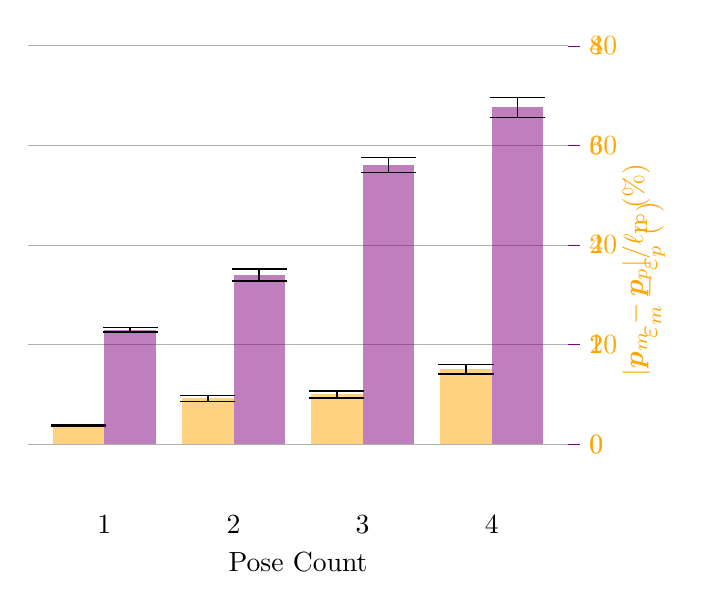
\begin{tikzpicture}
\definecolor{color0}{rgb}{1,0.647058823529412,0}
\definecolor{color1}{rgb}{0.501960784313725,0,0.501960784313725}
\begin{axis}[
anchor=origin,
axis line style={draw=none},
tick align=outside,
tick pos=both,
x grid style={white!69.01960784313725!black},
xmin=-0.59, xmax=3.59,
xtick style={color=black},
xtick style={draw=none},
xtick={0,1,2,3},
xticklabels={ , , , },
y grid style={white!69.01960784313725!black},
ylabel style={color=color0},
ylabel={\(\displaystyle |\bm{p}_m - \bm{p}_p|/\ell_{\textnormal{n}}\) (\%)},
ymin=-0.5, ymax=4,
ytick pos=left,
ytick pos=right,
ytick style={color=color0},
ytick style={color=color0},
yticklabel style={color=color0}
]
\draw[fill=color0,draw opacity=0,fill opacity=0.5] (axis cs:0,0) rectangle (axis cs:-0.4,0.191657134624049);
\draw[fill=color0,draw opacity=0,fill opacity=0.5] (axis cs:1,0) rectangle (axis cs:0.6,0.460290061670062);
\draw[fill=color0,draw opacity=0,fill opacity=0.5] (axis cs:2,0) rectangle (axis cs:1.6,0.502296434742686);
\draw[fill=color0,draw opacity=0,fill opacity=0.5] (axis cs:3,0) rectangle (axis cs:2.6,0.751151917563679);
\path [draw=black, semithick]
(axis cs:-0.2,0.183710156121145)
--(axis cs:-0.2,0.199604113126952);
\path [draw=black, semithick]
(axis cs:0.8,0.430868487068149)
--(axis cs:0.8,0.489711636271975);
\path [draw=black, semithick]
(axis cs:1.8,0.46807460565995)
--(axis cs:1.8,0.536518263825421);
\path [draw=black, semithick]
(axis cs:2.8,0.702731632174251)
--(axis cs:2.8,0.799572202953107);
\addplot [semithick, black, mark=-, mark size=10, mark options={solid}, only marks]
table {%
-0.2 0.183710156121145
0.8 0.430868487068149
1.8 0.46807460565995
2.8 0.702731632174251
};
\addplot [semithick, black, mark=-, mark size=10, mark options={solid}, only marks]
table {%
-0.2 0.199604113126952
0.8 0.489711636271975
1.8 0.536518263825421
2.8 0.799572202953107
};
\end{axis}
\begin{axis}[
anchor=origin,
axis line style={draw=none},
axis y line=right,
tick align=outside,
tick pos=both,
x grid style={white!69.01960784313725!black},
xlabel={Pose Count},
xmin=-0.59, xmax=3.59,
xtick style={color=black},
xtick style={draw=none},
xtick={0,1,2,3},
xticklabels={1,2,3,4},
y grid style={white!69.01960784313725!black},
ylabel style={color=color0},
ylabel={\(\displaystyle \varepsilon_m - \varepsilon_p\) (\(\displaystyle ^\circ\))},
ymajorgrids,
ymin=-10, ymax=80,
ytick pos=left,
ytick pos=right,
ytick style={color=color0},
ytick style={color=color1},
yticklabel style={color=color0}
]
\draw[fill=color1,draw opacity=0,fill opacity=0.5] (axis cs:0,0) rectangle (axis cs:0.4,23.0100920575588);
\draw[fill=color1,draw opacity=0,fill opacity=0.5] (axis cs:1,0) rectangle (axis cs:1.4,33.9783497479771);
\draw[fill=color1,draw opacity=0,fill opacity=0.5] (axis cs:2,0) rectangle (axis cs:2.4,56.0949000198084);
\draw[fill=color1,draw opacity=0,fill opacity=0.5] (axis cs:3,0) rectangle (axis cs:3.4,67.6191188302761);
\path [draw=black, semithick]
(axis cs:0.2,23.4160140765191)
--(axis cs:0.2,22.6041700385986);
\path [draw=black, semithick]
(axis cs:1.2,35.1783293382044)
--(axis cs:1.2,32.7783701577498);
\path [draw=black, semithick]
(axis cs:2.2,57.6024090509591)
--(axis cs:2.2,54.5873909886577);
\path [draw=black, semithick]
(axis cs:3.2,69.5990491995932)
--(axis cs:3.2,65.6391884609591);
\addplot [semithick, black, mark=-, mark size=10, mark options={solid}, only marks]
table {%
0.2 23.4160140765191
1.2 35.1783293382044
2.2 57.6024090509591
3.2 69.5990491995932
};
\addplot [semithick, black, mark=-, mark size=10, mark options={solid}, only marks]
table {%
0.2 22.6041700385986
1.2 32.7783701577498
2.2 54.5873909886577
3.2 65.6391884609591
};
\end{axis}
\end{tikzpicture}
%% End matplotlib2tikz content %% 
\end{document}